\documentclass{article}
% these lines load any packages you might wish to use. 
% some common ones are loaded below
\usepackage{amsfonts, amsmath, amssymb}
\usepackage[numbers,square,sort&compress]{natbib}
\usepackage{graphicx}  % required for inserting images
\usepackage{hyperref}  % for inserting urls, and having clickable links to equation and figure numbers
\usepackage[margin=1.2 in]{geometry}  % these margins are easy to read
\geometry{letterpaper}                   % ... or a4paper or a5paper or ... 
\usepackage{lmodern}		% good font
\usepackage{caption} % for \captionsetup
\usepackage{appendix}
\usepackage{subcaption}
\usepackage{graphicx}
\usepackage{float}
\usepackage{hyperref}

\usepackage{tikz}  % for using tikz, to draw your own figures
\usetikzlibrary{angles,quotes}

% input document information here
\title{Time distribution of finding a wallet in a room}
\author{Ryan Hsiao 61609715, Fanbo Feng 95719241, Davis Li 49877293}
\date{}  % if you uncomment this, it will not put the date.
%\date{Dec 99, 1999}   % if you uncomment this, it will list the date as whatever is inside the curly brackets


\begin{document}

\maketitle


\section{Introduction}
In everyday life, people often spend time searching for misplaced items, such as a lost wallet or keys, inside their homes. The time required to locate an item depends on many factors, including the layout of the room and the efficiency of a search strategy. Because human search behavior can involve random exploration, stochastic models provide a useful framework for studying such processes. 

\vspace{5mm}

\noindent To analyze this problem, we model the room as a two-dimensional region containing several obstacles that restrict the movement of the searcher. A searcher begins from a fixed starting point and moves continuously within the accessible region until the object is found. We simulate the motion of the person searching for the wallet using two different strategies. The first strategy models the searcher’s motion as a random walk based on Brownian motion, representing an entirely random search behavior. The second strategy resembles the movement of a robot vacuum, in which the searcher moves in a fixed direction until encountering a boundary and then changes direction randomly.

\vspace{5mm}

\noindent Using numerical simulations, we generate a large number of search trials for different wallet locations within the room. The resulting search times are then analyzed using probability distributions and summary statistics in order to interpret the characteristics of the search process. By comparing the distributions of search times for the two strategies, we aim to identify how movement patterns influence the efficiency of locating an object.

\section{Model}\label{sec:model}
\subsection{Definitions and Notations}
\noindent We consider a person searching for a lost object inside a house, which is modeled as a two-dimensional region with fixed obstacles. The searcher moves continuously until the object is found.

\vspace{5mm}

%%%%%%%%%%%%%%%%%%%%%%%%%%%%%%%%%%%%%%%%%% Table start
\begin{table}[!h]
\begin{center}
\begin{tabular}{||c | c | c | c||} 
 \hline
 Symbol & Description & Type & Dimensions \\ [0.3ex] 
 \hline\hline
 $X$ & The horizontal position of the person & Dependent Variable & L \\ 
 \hline
 $Y$ &  The vertical position of the person & Dependent Variable & L \\ 
 \hline
 $W_1$ & The horizontal component of Brownian motion  & Random Variable & T$^{-\frac{1}{2}}$ \\ 
 \hline
 $W_2$ & The vertical component of Brownian motion  & Random Variable & T$^{-\frac{1}{2}}$ \\ 
 \hline
 $\sigma$ & The parameter describing how fast the person diffuse& Parameter & LT$^{-\frac{1}{2}}$ \\ 
 \hline
 $v$ & The speed of the person walking in the house & Parameter & LT$^{-1}$ \\ 
 \hline
 $\theta$ & Movement angle & Random variable & -- \\ 
 \hline
 $t$ & Time & Independent Variable & T \\ 
 \hline
 $\Omega$ & Accessible area of the room & Set & -- \\ 
 \hline
\end{tabular} 
\end{center}
\captionsetup{font=small}
\caption{The variables and parameters are measured in \textit{seconds} ($s$, dimension T) and \textit{meters} ($m$, dimension L).} % All dimensions L has the unit of meter, and dimensions of T has the unit of second.
\end{table}
%%%%%%%%%%%%%%%%%%%%%%%%%%%%%%%%%%%%%%%%%% Table end

\noindent The goal of the model is to analyze the distribution of the time required to locate a lost wallet inside a room. The room is represented from a bird’s-eye view, where the wallet is assumed to be fixed at an unknown location. The search domain $\Omega$ represents the accessible area of the room in which the searcher can move, while regions occupied by fixed obstacles such as furniture or walls are excluded from this region. Thus, the position of the searcher at time $t$ is given by the vector 
\begin{align*}
    (X(t), Y(t)) \in \Omega \ .
\end{align*}
Since we consider a realistic movement pattern, we assume $t > 0$ and $\theta \sim \text{Unif}(0, 2\pi]$. Position is measured in meters (m) and time is measured in seconds (s) (Table 1).

\vspace{5mm}

\noindent The house map is based on the typical layout of a living room (Figure 1). We consider the circle in the lower left of the map as the dining table, the larger rectangle above it as the sofa, the small rectangle above the sofa as the TV bench, and the rectangle on the right side of the map as the kitchen table. The small orange circles with a triangle inside are considered as the positions of the lost item, and the green cross represents the starting point of the person.

%%%%%%%%%%%%%%%%%%%%%%%%%%%%%%%%%%%%%%%%%% Plot Start
\begin{figure}[!h]
\centering
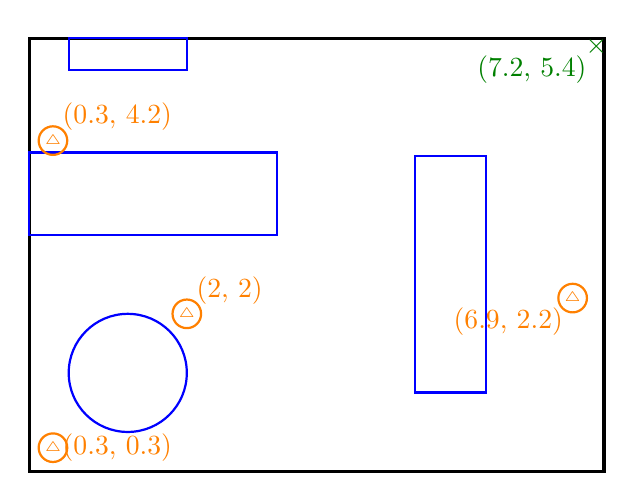
\begin{tikzpicture}[scale=1, >=stealth]
    % Main Boundary Box (Black)
    \draw[very thick] (0,0) rectangle (7.3, 5.5);

    % Blue Shapes
    \draw[blue, thick] (0.5, 5.1) rectangle (2, 5.5); % Top rectangle
    \draw[blue, thick] (0, 3) rectangle (3.15, 4.05); % Middle left rectangle
    \draw[blue, thick] (1.25, 1.25) circle (0.75);     % Bottom left circle (est. radius)
    \draw[blue, thick] (4.9, 1) rectangle (5.8, 4);   % Tall right rectangle

    % Orange Triangle Icons and Coordinates
    \newcommand{\orangeicon}[1]{
        \node[draw, orange, thick, circle, inner sep=1pt] at #1 {\tiny $\triangle$};
    }
    
    \orangeicon{(0.3, 4.2)}
    \node[orange, above right] at (0.3, 4.2) {(0.3, 4.2)};
    
    \orangeicon{(0.3, 0.3)}
    \node[orange, right] at (0.3, 0.3) {(0.3, 0.3)};
    
    \orangeicon{(2, 2)}
    \node[orange, above right] at (2, 2) {(2, 2)};
    
    \orangeicon{(6.9, 2.2)}
    \node[orange, below left] at (6.9, 2.2) {(6.9, 2.2)};

    % Green "X" and Coordinate
    \node[green!50!black, thick] at (7.2, 5.4) {$\times$};
    \node[green!50!black, below left] at (7.2, 5.4) {(7.2, 5.4)};
\end{tikzpicture}
\captionsetup{font=small}
\caption{Bird's eye view of the living room, region $\Omega$. For future reference, we define the following: point 1 (0.3, 4.2), point 2 (2, 2), point 2 (6.9, 2.2), and point 4 (0.3, 0.3).}
\label{fig:placeholder}
\end{figure}
%%%%%%%%%%%%%%%%%%%%%%%%%%%%%%%%%%%%%%%%%% Plot End

\noindent We determine the set parameter for the accessible area $\Omega$ by establishing a coordinate system on the map of the house shown in Figure 1 above. We define the lower-left corner of the map as the origin, with the bottom wall representing the $x$-axis and the left wall representing the $y$-axis. We consider four possible locations for the lost item, given by coordinates (0.3, 4.2), (2.0, 2.0), (6.9, 2.2), (0.3, 0.3), and the starting point with coordinate (7.2, 5.4). Returning to $\Omega$, we first define the sets corresponding to the house and the obstacles. The entire house area, TV bench, sofa, kitchen table, and dining table are denoted by $R_{room},\ R_1,\ R_2,\ R_3$, and $C_1$, respectively:
\begin{align*}
R_{room} &=\{(x,y) \in \mathbb{R}^2\mid 0 \le x \le 7.3 \ , 0 \le y \le 5.5\} \\
R_1 &= \{(x,y) \in \mathbb{R}^2\mid 0.6 \le x \le 2.4 \ , 5.05 \le y \le 5.5 \} \\
R_2 &= \{(x,y) \in \mathbb{R}^2\mid 0 \le x \le 3 \ , 3.15 \le y \le 4.05 \} \tag{2.1} \\
R_3 &= \{(x,y) \in \mathbb{R}^2\mid 4.9 \le x \le 5.8 \ , 1 \le y \le 4 \} \\ 
C_1 &= \{(x,y) \in \mathbb{R}^2\mid (x - 1.25)^2 + (y-1.25)^2 \le 0.75^2 \} .
\end{align*}
Hence, we can compute $\Omega$:
$$
\Omega = R_{room} \backslash (R_1 \cup R_2 \cup R_3 \cup C_1),
$$
which represents the walkable area in the house with the predetermined layout.

\vspace{5mm}

\noindent We select the points (0.3, 4.2) and (6.9, 2.2) to examine how the width of the pathways between obstacles affects the search time. The former is located in a region with a narrower passage, while the latter is more accessible with a wider path. We also include the points (0.3, 0.3) and (2.0, 2.0), where the difficulty of reaching the target varies due to the arrangement of surrounding obstacles. These points provide additional comparisons with different levels of accessibility. 

\vspace{5mm}

\noindent Next, we assume conditions to simplify the model from a real world scenario in order to achieve the target model mentioned above. First, the action takes place in a two-dimensional indoor setting. Furthermore, the person continuously moves within the accessible region $\Omega$, and obstacles such as furniture act as impenetrable boundaries. Finally, when a person bumps into a wall or obstacle, their movement will be deflected, and then walks off in a random direction. In addition, the movement speed of the person and the position of the object are fixed and will not change over time. The person continues moving until the object is found without receiving help from anyone or anything. These assumptions allow the searcher's motion to be represented using stochastic movement rules.

\subsection{Strategy 1: Random Walk Search}

\noindent In our first strategy, the searcher moves randomly inside the room, representing an unguided search behavior. The motion is modeled by stochastic differential equations (SDEs) respective to changes in horizontal and vertical displacements:
\begin{align*}
    \begin{cases}
        \mathrm{d}X = \sigma \mathrm{d}W_1, \\
        \\
        \mathrm{d}Y = \sigma \mathrm{d}W_2,
    \end{cases}   \tag{2.2}
\end{align*}
\noindent where $\sigma > 0$ measures the diffusion rate of the person, and $W_1(t)$ and $W_2(t)$ are independent Brownian motions [2]. 

\vspace{5mm}

\noindent This strategy captures continuous random fluctuations in both directions, resulting in a highly irregular and exploratory search path.


\subsection{Strategy 2: Directed Random Motion (Robot Vacuum)}

\noindent Our second strategy resembles the motion of a robot vacuum. Here, the searcher travels in a fixed direction until encountering a boundary.

\vspace{5mm}

\noindent The motion is described by a system of ordinary differential equations (ODEs):
\begin{align*}
    \begin{cases}
        \mathrm{d}X = v \cos(\theta)\mathrm{d}t, \\
        \\
        \mathrm{d}Y = v \sin(\theta)\mathrm{d}t,
    \end{cases}   \tag{2.3}
\end{align*}

\noindent where $v > 0$ is the magnitude of the searcher's speed, and $\theta \sim \text{Unif}(0, 2\pi]$ is the angle that determines the direction of motion. 

\vspace{5mm}

\noindent This strategy represents a more structured movement pattern, where the searcher maintains a constant direction between changes.

\subsection{Comparison of the Strategies}
\noindent The two strategies fundamentally differ in both the mathematical structures of their governing equations and their resulting search behaviors.

\vspace{5mm}

\noindent Strategy 1 is a purely diffusive process described by SDEs (2.2). The direction changes randomly and continuously over time, producing irregular paths that do not follow any consistent direction. In contrast, Strategy 2 is described by a system of ODEs (2.3). The searcher moves in a fixed direction at a constant speed until the direction changes, at which point a new angle $\theta$ is sampled. This results in straight paths interrupted by occasional random turns.

\vspace{5mm}

\noindent The key difference between the two strategies is directional persistence: Strategy 1 has no persistence in its movement, while Strategy 2 maintains a fixed direction over short periods of time. As a result, Strategy 1 tends to keep the searcher near the same area, whereas Strategy 2 allows the searcher to travel farther before changing direction.

\subsection{Numerical Simulations}
In this section, we approximate solutions to the SDEs of Strategy 1 and ODEs of Strategy 2 using equations (2.2) and (2.3). Since we are interested in the search time of each strategy, we do not set the time interval and steps required. Instead, we set a fixed discrete time step $\mathrm{d}t$. To obtain the value of $\mathrm{d}t$, we choose a sufficiently small time step $\mathrm{d}t = 0.01$ so that the simulation remains consistent. In our case, consistency indicates that the searcher does not step outside of $\Omega$ and the strategies follow their characteristic motion, as shown in Figure 2. 

\subsubsection*{Strategy 1: Brownian Motion}
\noindent The Wiener process (Brownian motion) is a continuous stochastic process $W(t)$ that describes random motion over time. From $W(0) = 0$, it increments over time intervals $\mathrm{d}t$, which are normally distributed with mean $0$ and variance $\mathrm{d}t$.

\vspace{5mm}

\noindent To simulate this process numerically, we approximate it using a discrete time step. At each step, we generate independent standard normal random variables $\eta_k \sim \mathcal{N}(0,1)$ for $k=0, 1, \dots , N-1$. Hence, the Wiener process [2] can then be approximated recursively by
\begin{align*}
     W_{k+1} = W_k + \sqrt{\mathrm{d}t}\, \eta_k \ , \ \ k=0,1,\dots,N-1.  
\end{align*}

\noindent Subsequently, we simulate the SDEs (2.2) with Wiener process by approximating the continuous variables $X$ and $Y$ using discrete positions $\mathrm{d}X = X_{n+1} - X_n$, $\mathrm{d}Y = Y_{n+1} - Y_n$, where the index $n$ represents the current position and $n+1$ represents the position at the next iteration. Under this discretization, the increments are given by
\begin{align*}
    \begin{cases}
        X_{n+1} = X_n + \eta_n\sqrt{\mathrm{d}t}, \\
        \\
        Y_{n+1} = Y_n + \eta_n\sqrt{\mathrm{d}t}.
    \end{cases}
\end{align*}

\subsubsection*{Strategy 2: Robot Vacuum Motion}
\noindent The searcher moves in the same direction (a straight line) as long as the position $(X, Y)$ is an accessible area in $\Omega$. If the proposed position results outside the accessible area of the room such as inside a furniture or out of room boundary, i.e. $(X, Y) \notin \Omega$, a new direction is chosen by sampling an angle from the uniform distribution $\theta \sim \text{Unif}(0, 2\pi]$. 

\vspace{5mm}

\noindent Similar to the discretization process above, the increments are given by 
\begin{align*}
    \begin{cases}
        X_{n+1} = X_n + v\cos(\theta)\mathrm{d}t, \\
        \\
        Y_{n+1} = Y_n + v\cos(\theta)\mathrm{d}t.
    \end{cases}
\end{align*}

\subsubsection*{Simulation process}
We use a while loop to check whether the searcher is inside the circle of the targeted location. If $(X, Y)\in\text{target}$, we consider the wallet to be found. If $(X, Y)\notin\text{target}$, the searcher continues to perform a random walk. During the process, we check the position of the searcher and make the searcher perform corresponding actions while reaching the boundary of $\Omega$. We repeat this process until the wallet is found. The code is available in the \href{https://github.com/tusm06/MATH461_Unit03}{Git Repository}.

\section{Results}
\subsection{Assigning Values to Parameters}
In order to compare the two strategies, the scalar speed for both should be the same. We also know that the value for the person walking in a house is approximately $1.31\ m/s$ [1]. Although the speed value from the article is measured in the outdoors, we assume that the person walks in a constant speed in all environments. This magnitude of speed can be directly used in Strategy 2 because it can be divided into horizontal and vertical components with a given angle. However, for Strategy 1, we cannot directly use this speed in a SDE because $\sigma$ describes how fast the person diffuses in the house rather than how fast the person walks. 

\vspace{5mm}

\noindent To ensure both strategies have the same scalar speed, we need to calculate the diffusion coefficient based on the speed value we have. Then, we use this coefficient to compute the value of $\sigma$. We define the diffusion coefficient with the symbol $D$, and we can obtain the relation between $\sigma$ and $D$ from lecture notes, which is $D=\dfrac{1}{2}\sigma^2$ [2]. From ``Random Walks in Biology", we know that the square of the distance in two-dimensional random walk can be calculated by the diffusion coefficient, $D$, with the equation $\langle r^2 \rangle = 4D\tau$, where $r$ is the distance moved in time $\tau$ [3]. Since $\langle r^2 \rangle$ is the expected value of the squared distance traveled, we set this expectation equal to $d^2$, where $d$ denotes the expected distance traveled in time $\tau$. This gives
\begin{align}
    d^2 = 4D\tau. \tag{3.1}
\end{align}


\noindent Next, we write the $d^2$ in terms of the scalar speed:
\begin{align}
    d^2 = (v\tau)^2=v^2\tau^2. \tag{3.2}
\end{align}


\noindent Lastly, we substitute (3.2) and $D$ into (3.1):
\begin{align}
    v^2\tau^2 = 2 \sigma^2\tau.  \tag{3.3}
\end{align}

\noindent For Strategy 2, we already have the scalar speed $v = 1.31\ m/s$, which means the searcher can walk $1.31\ m/s$. Thus, the scalar speed for Strategy 2 is the distance moved in one second.To ensure the scalar speed for Strategy 1 also describes the distance moved in one second, the traveling time $\tau$ must be 1 s. Hence, we can solve equation (3.3) and obtain the value of $\sigma$ by plugging in $v = 1.31$ and $\tau  = 1$. Since we set $d = v\tau$ and  $\tau = 1$, the distance traveled in one second is $d = v$. This ensures that the person travels in the same distance per second as in Strategy 2, so both strategies have the same scalar speed. As a result, we can compute $\sigma$ as follows:
\begin{align*}
    \sigma = \sqrt{\frac{v^2\tau}{2}} \approx 0.926 ,
\end{align*}
where the unit of $\sigma$ is meters per square root of seconds ($\dfrac{m}{\sqrt{s}}$).


\subsection{Computing Results for the Two Strategies}
Using the parameter values assigned above, we can compute our results following our numerical simulations and visualize them with box plots and trajectory plots. In the trajectory plots, we simulate the layout of the house, which shows the person's walk path during the process on a simulated map. The box plots provide statistical information for the search time elapsed over all trials.

\subsubsection{Visualizing the Walking Path in the Finding Process}
For each strategy, we run 5000 trials on each of the four item locations. We then save the first trial and plot its path for visualization. In the trajectory plots, obstacles are represented by rectangles and circles outlined with dashed blue lines, while the walls are shown as black solid lines forming the boundary of the room. The position of the lost item is indicated by an orange dashed circle, and the orange point within it marks the location where the item is found. The other orange point in the upper-right corner represents the starting position of the searcher, and the path traveled during the search is displayed as solid green lines.

%%%%%%%%%%%%%%%%%%%%%%%%%%%%%%%% Begin plots %%%%%%%%%%%%%%%%%%%%%%%%%%%%%%%%%%%%%
\begin{figure}[H]
     \centering
     % --- First Row ---
     \begin{subfigure}[b]{0.45\textwidth}
         \centering
         
\includegraphics[width=\textwidth]{image/S1P4_Path.png}
          \captionsetup{font=small}
         \caption{Strategy 1 path, both X and Y in meters (m)}
     \end{subfigure}
     \hfill
     \begin{subfigure}[b]{0.45\textwidth}
         \centering
         
\includegraphics[width=\textwidth]{image/S2P2_Path.png}
         \captionsetup{font=small}
         \caption{Strategy 2 path, both X and Y in meters (m)}
     \end{subfigure}
     \captionsetup{font=small}
     \caption{In this figure, we show the simulated paths of the two strategies, where plot (a) is Strategy 1 (Brownian motion) and plot (b) is Strategy 2 (robot vacuum motion).}
     \label{fig:four_plots}
\end{figure}
%%%%%%%%%%%%%%%%%%%%%%%%%%%%%%%% End plots %%%%%%%%%%%%%%%%%%%%%%%%%%%%%%%%%%%%%

\noindent Together, we have 8 trajectory plots, and each strategy has 4 plots. We show one of our results in Strategy 1 and Strategy 2 respectively in Figure 2 above. The left plot shows the searcher’s movement under Brownian motion, while the right plot shows the movement under the directed motion strategy.

\vspace{5mm}

\noindent We only show two trajectory plots because other plots with the same strategy cannot provide more information. These plots show only one trial for each situation that is a completely random process. Thus, there is not much value in comparing the different trajectory plots under the same strategy, so we choose these two plots to show the difference of the path from different strategies.

\subsubsection{Statistical Information for the Two Strategies}

Unlike trajectory plots, bar charts can provide the distribution of the results from all 5000 simulation trials for each target position under a given strategy. We compute four bar charts for each strategy to compare search time in different situations. However, most of the searching time results are exponential distributions, only two of them are Gamma distributions, which are quite similar to exponential distributions as they are slightly left skewed. We cannot get much valuable information from the bar charts. 

\vspace{5mm}

\noindent To obtain more statistics, we use box plots since the distributions are either exponential or gamma, which are asymmetric and right-skewed. We summarize the results using the median and the interquartile range (IQR). In addition, the median and IQR are less sensitive to outliers compared to the mean and variance. Considering that the distribution is skewed and with a wide range of search times, potential outliers can influence the statistic. Hence, we look at the statistics with the box plots as in Figures 3 and 4 below, which characterized the statistics for the search time.

\subsubsection*{Results for Strategy 1 (Brownian Motion)}

%%%%%%%%%%%%%%%%%%%%%%%%%%%%%%%% Begin plots %%%%%%%%%%%%%%%%%%%%%%%%%%%%%%%%%%%%%
\begin{figure}[H]
     \centering
     % --- First Row ---
     \begin{subfigure}[b]{0.8\textwidth}
         \centering
         
\includegraphics[width=\textwidth]{image/box-plot_S1.png}
     \end{subfigure}
     \captionsetup{font=small}
     \caption{Time distribution for different wallet locations using Strategy 1 (Brownian motion). The bottom of the rectangle represents the $25\%$ quantile and the top represents the $75\%$ quantile. The orange line is the median and the hollow dots at the upper end represent potential outliers. Time is scaled from 0 to 2500 s for better visualization.}
     \label{fig:four_plots}
\end{figure}
%%%%%%%%%%%%%%%%%%%%%%%%%%%%%%%% End plots %%%%%%%%%%%%%%%%%%%%%%%%%%%%%%%%%%%%%

We compute the results for Strategy 1 using four different target positions, as shown in Figure 3. The box plots summarize the distribution of search times. Since the data are right-skewed, we focus on the median and interquartile range (IQR) reported in Table 2. From the results, we observe that the search times for Points 2 and 3 are generally shorter than those for Points 1 and 4.

%%%%%%%%%%%%%%%%%%%%%%%%%%%%%%%% Begin Table %%%%%%%%%%%%%%%%%%%%%%%%%%%%%%%%%%%%%
\begin{table}[h]
\centering
\label{tab:time_stats_s2}
\begin{tabular}{c|c|c|c|c}
\textbf{Locations} & \textbf{25\%} & \textbf{median} & \textbf{75\%} & \textbf{IQR} \\ \hline
Point 1: $(0.3, 4.2)$ & 75.260 & 177.210 & 358.075 & 282.815 \\ 
Point 2: $(2.0, 2.0)$ & 33.408 & 61.455 & 107.222 & 73.815 \\ 
Point 3: $(6.9, 2.2)$ & 7.775 & 22.290 & 80.165 & 72.390 \\ 
Point 4: $(0.3, 0.3)$ & 75.990 & 156.920 & 283.857 & 207.867 \\
\end{tabular}
\captionsetup{font=small}
\caption{Statistic summaries of Strategy 1 with different wallet locations. Where $IQR = 75\% - 25\%$. This table shows detailed key values for Figure 3. All values in this table are measured in seconds.}
\end{table}
%%%%%%%%%%%%%%%%%%%%%%%%%%%%%%%% End Table %%%%%%%%%%%%%%%%%%%%%%%%%%%%%%%%%%%%%

\subsubsection*{Results for Strategy 2 (Robot Vacuum Motion)}


%%%%%%%%%%%%%%%%%%%%%%%%%%%%%%%% Begin plots %%%%%%%%%%%%%%%%%%%%%%%%%%%%%%%%%%%%%
\begin{figure}[H]
     \centering
     % --- First Row ---
     \begin{subfigure}[b]{0.8\textwidth}
         \centering
         
\includegraphics[width=\textwidth]{image/box-plot_S2.png}
     \end{subfigure}
     \captionsetup{font=small}
     \caption{Time distribution for different wallet locations using Strategy 2 (robot vacuum motion). The bottom of the rectangle represents the $25\%$ quantile and the top represents the $75\%$ quantile. The orange line is the median and the hollow dots at the upper end represent potential outliers. Time is scaled from 0 to 1300 s for better visualization.}
     \label{fig:four_plots}
\end{figure}
%%%%%%%%%%%%%%%%%%%%%%%%%%%%%%%% End plots %%%%%%%%%%%%%%%%%%%%%%%%%%%%%%%%%%%%%


\noindent Similarly, we compute the results for Strategy 2 based on four different target positions and demonstrate them in the form of box plots as in Figure 4. We summarize the statistical information of the results in the same way as we did for Strategy 1, as shown in Table 3. Now we see that the search times for point 2 and point 3 are still relatively less than the times for point 1 and point 4. However, the difference between them is not as significant as that we have seen in Strategy 1 scenarios.


%%%%%%%%%%%%%%%%%%%%%%%%%%%%%%%% Begin Table %%%%%%%%%%%%%%%%%%%%%%%%%%%%%%%%%%%%%
\begin{table}[h]
\centering
\label{tab:time_stats_s2}
\begin{tabular}{c|c|c|c|c}
\textbf{Locations} & \textbf{25\%} & \textbf{median} & \textbf{75\%} & \textbf{IQR} \\ \hline
Point 1: $(0.3, 4.2)$ & 27.377 & 75.115 & 161.475 & 134.097 \\ 
Point 2: $(2.0, 2.0)$ & 29.905 & 60.795 & 115.735 & 85.830 \\ 
Point 3: $(6.9, 2.2)$ & 8.007 & 30.895 & 73.100 & 65.093 \\ 
Point 4: $(0.3, 0.3)$ & 38.367 & 80.605 & 149.157 & 110.790 \\
\end{tabular}
\captionsetup{font=small}
\caption{Statistic summaries of Strategy 2 with different wallet locations. Where $IQR = 75\% - 25\%$. This table shows detailed key values for Figure 4. All values in this table are measured in seconds.}
\end{table}
%%%%%%%%%%%%%%%%%%%%%%%%%%%%%%%% End Table %%%%%%%%%%%%%%%%%%%%%%%%%%%%%%%%%%%%%

\section{Discussion}
\subsubsection*{Effect of wallet locations on search time}
Based on the search times shown in Figures 3 and 4, we observe that when the wallet is located at points 1 and 4, the search times are significantly greater than those at points 2 and 3. This can be due to the arrangement of the furniture, as points 1 and 4 lie in narrower regions that are more difficult to access. Although the potential outliers in Figures 3 and 4 appear to have a large difference, the median and IQR for these points are similar, as shown in Tables 2 and 3. This indicates that points 1 and 4 have comparable levels of search difficulty. While it may seem unrealistic that a searcher would have trouble navigating a narrow passage, the searcher may fail to enter or fully explore such regions under a ``random walk''. This behavior can be observed in the trajectory plots in Figure 2.

\vspace{3mm}

\noindent On the other hand, the search times for points 2 and 3 are generally shorter, with both the median and IQR significantly smaller than those for points 1 and 4 across both strategies. This is likely because these points are located in more open areas, making them easier for the searcher to reach. Among them, point 2 typically takes a longer search time than point 3 under both strategies. This can be explained by the arrangement of the furniture, as there are obstacles between the starting point and the wallet location at point 2.

\subsubsection*{Effect of strategy on search time}
From the plots in Figure 2, we observe that Strategy 1 tends to revisit the same areas more frequently, whereas Strategy 2 is less likely to do so. As a result, Strategy 2 generally leads to shorter search times for points 1 and 4. However, since points 2 and 3 are located in relatively open areas as discussed above, the difference between the two strategies is less significant.


% Why p1 and p4 required more search time. due to complicated path to reach due to arrange of the furnature. 
% p2 and p3 are in open area
% S2 is more likely to find the wallet as it do not waste time to search repeated places.aq



\section{Conclusion}
In this project, we developed a stochastic model to investigate the time required to find a lost wallet inside a furnished room. The room was represented as a two-dimensional domain with an accessible area $\Omega$, and two search strategies were considered: a random walk modeled by Brownian motion and a directed motion resembling the movement of a robot vacuum. Numerical simulations were performed to analyze the search time distributions for different wallet locations. Our results show that the search time distributions are generally right-skewed, meaning that most trials ended up finding the wallet quickly while a small number required much longer search times. By comparing the two strategies, directed motion tends to perform better when the wallet is located in areas that are harder to access due to obstacles, whereas the random walk strategy could locate the wallet more efficiently when the wallet's location is relatively open. These results highlight how both the choice of search strategy and the spatial arrangement of obstacles influence the efficiency of locating a lost object.


%%%%%%%%%%%%%%%%%%%% Refrence Start %%%%%%%%%%%%%%%%%%%%%%%%%%%
\bibliographystyle{plain} % you can choose from many different styles: https://www.overleaf.com/learn/latex/Bibtex_bibliography_styles
\begin{thebibliography}{2} % Entries are in the Refs.bib file
\bibitem[1]{one}
Elaine M. Murtagh, Jacqueline L. Mair, Elroy Aguiar, Catrine Tudor-Locke, and Marie H. Murphy. Outdoor Walking Speeds of Apparently Healthy Adults: A Systematic Review and Meta-analysis. Sports Medicine, 51, 125–141, 2021.
\bibitem[2]{two}
Miranda Holmes-Cerfon. Stochastic Modelling: Monte Carlo Sampling, and a bit of  Mathematical Finance. MATH 461, University of British Columbia. 2026.
\bibitem[3]{three}
Howard C. Berg. Random Walks in Biology. Princeton University Press, Princeton. 6-11, 1993.

\end{thebibliography}
%%%%%%%%%%%%%%%%%%%% Reference end %%%%%%%%%%%%%%%%%%%%%%%%%%%%%
\newpage

\section*{Gen AI declaration} 
Generative AI tools including ChatGPT and Grok were used as study aids for this project. They were used to help clarify ecological and mathematical concepts about predator-prey models and locate relevant research articles.

\vspace{5mm}

\noindent All mathematical models, parameters, analysis, simulations, figures, and conclusions were developed and verified independently by the authors. All equations, assumptions, and results presented in this report reflect our own understanding. The final report was reviewed and edited by the authors to ensure accuracy, precision, and clarity.

\end{document}
